\documentclass[a4paper,12pt]{article}
\usepackage{setspace}
\usepackage{amsmath}
\usepackage{courier}
\let\openbox\relax
\usepackage{newtxtext,newtxmath}
\usepackage{algorithm}
\usepackage{algpseudocode}
\usepackage{hyperref}
\usepackage{booktabs}
\usepackage{longtable}
\usepackage{graphicx}
\usepackage{caption}
\usepackage{subcaption}

% 调整章节标题字体大小
\usepackage{titlesec}
\titleformat{\section}{\Large\bfseries}{\thesection}{1em}{}
\titleformat{\subsection}{\large\bfseries}{\thesubsection}{1em}{}
\titleformat{\subsubsection}{\normalsize\bfseries}{\thesubsubsection}{1em}{}

\title{\textbf{Practice 8}}

\author{\textbf{Yanqiao Chen}\\
        Department of Computer Science and Engineering\\
        Southern University of Science and Technology\\
        \texttt{12412115@mail.sustech.edu.cn}}


\setstretch{1}   % 自定义行距（1.3倍）

\begin{document}

\maketitle

\tableofcontents

\section{Task 1}

The data is plotted as follows: 

\begin{center}
    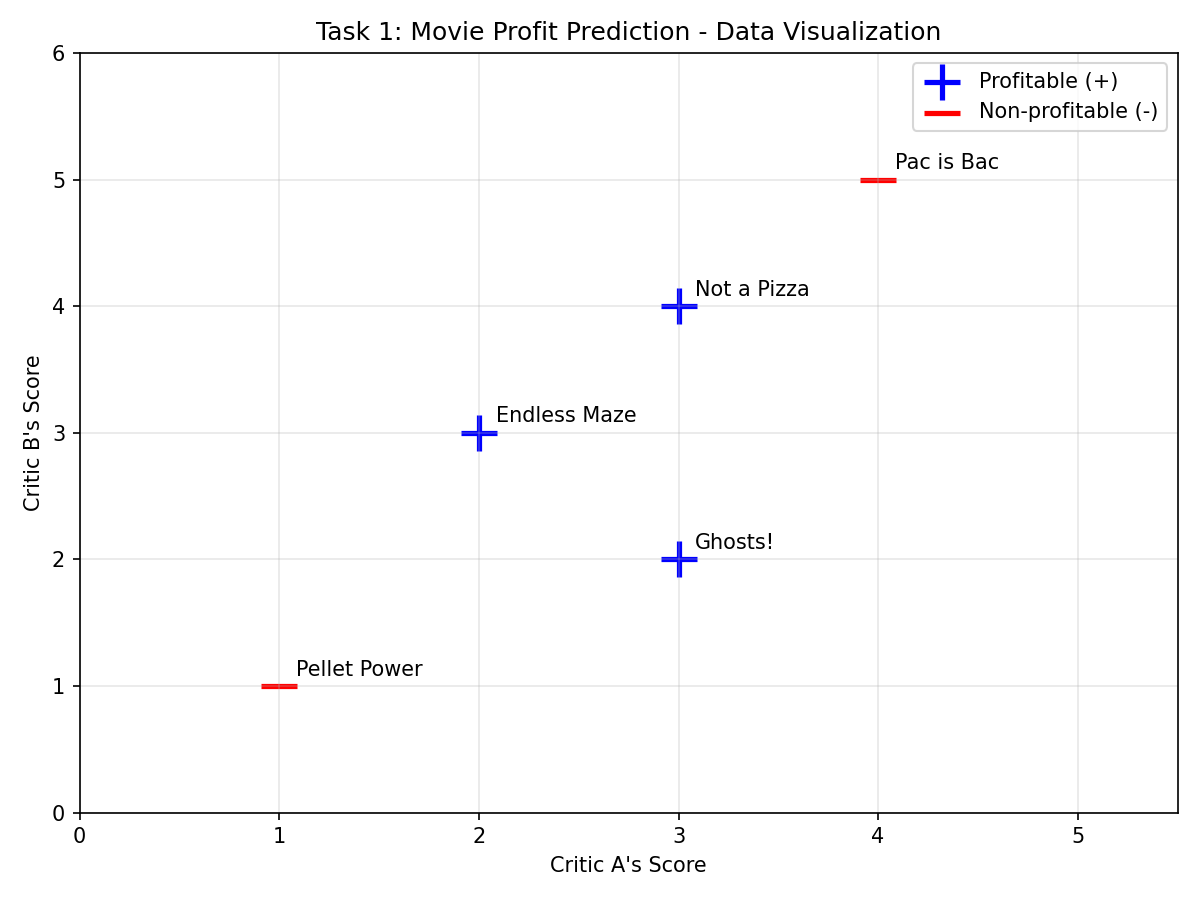
\includegraphics[width=0.8\textwidth]{task1_plot.png}
\end{center}

Trivally, this data is not linearly separable in 2D space. Thus SVM with linear kernel will not work well. Using RBF kernel may work better.

For NN, we can use a non-linear feedforward neural network with one hidden layer to classify the data. However, this dataset is very small, so we need to be careful to avoid overfitting. But a linear perceptron will not work well as it can only learn linear decision boundaries.

For Decision Tree, the task is appropriate as it can handle non-linear decision boundaries. We can use a simple decision tree classifier to classify the data.

In conclusion, Decision Tree may be the best choice as it is simple and effective for this type of data. SVM with RBF kernel can also work well, but it may require more tuning of hyperparameters. NN may not be the best choice due to the small size of the dataset, and it is more complex than the other two methods.

\section{Task 2}

\subsection{Perceptron Model Training and Feature Selection}

We use features $\mathbf{x} = [f_0, f_1, f_2]$, where $f_0 = 1$ (bias), $f_1 = \text{A's score}$, and $f_2 = \text{B's score}$. The dataset with labels ($+1$ for Yes, $-1$ for No) is:

\begin{center}
\begin{tabular}{lccc}
\toprule
\textbf{Movie Name} & $f_1$ (A) & $f_2$ (B) & \textbf{Label} \\
\midrule
Pellet Power  & 1 & 1 & $-1$ \\
Ghosts!       & 3 & 2 & $+1$ \\
Pac is Bac    & 4 & 5 & $-1$ \\
Not a Pizza   & 3 & 4 & $+1$ \\
Endless Maze  & 2 & 3 & $+1$ \\
\bottomrule
\end{tabular}
\end{center}

\subsubsection{Weight Update Rule}

For each sample, compute the prediction:
\[
\hat{y} = \text{sign}(\mathbf{w} \cdot \mathbf{x})
\]
If the prediction is wrong ($\hat{y} \neq y_{\text{true}}$), update the weights:
\[
\mathbf{w} \leftarrow \mathbf{w} + \eta \cdot y_{\text{true}} \cdot \mathbf{x}
\]
If correctly classified, do nothing. Here we use learning rate $\eta = 1$ and initial weights $\mathbf{w} = [0, 0, 0]$.

\subsubsection{First Weight Update}

\begin{itemize}
    \item \textbf{Sample 1} (Pellet Power): $\mathbf{w} \cdot \mathbf{x} = 0$. With $\text{sign}(0) = -1$, the prediction matches the true label $-1$. \textbf{No update}.
    \item \textbf{Sample 2} (Ghosts!): $\mathbf{w} \cdot \mathbf{x} = 0$, $\text{sign}(0) = -1 \neq +1$. \textbf{Misclassified}.
\end{itemize}

Apply the update rule:
\[
\mathbf{w}_{\text{new}} = \mathbf{w} + \eta \cdot y \cdot \mathbf{x} = [0,0,0] + 1 \cdot (+1) \cdot [1, 3, 2] = \mathbf{[1,\ 3,\ 2]}
\]

\textbf{After the first update:} $\mathbf{w} = [1, 3, 2]$, i.e., $w_0 = 1$, $w_1 = 3$, $w_2 = 2$.

\subsection{Scenario Analysis}

We discuss whether a perceptron with the given features can perfectly classify three hypothetical scenarios.

\subsubsection{Scenario (i): $A + B > 8$}

\textbf{Conclusion: Yes, linearly separable.}

The rule $A + B > 8$ corresponds to a linear decision boundary:
\[
-8 + A + B = 0
\]
A perceptron can implement this exactly with weights $\mathbf{w} = [-8, 1, 1]$.

\subsubsection{Scenario (ii): $A \in \{2,3\}$ and $B \in \{2,3\}$}

\textbf{Conclusion: No, not linearly separable.}

The YES points form a solid square: $\{(2,2), (2,3), (3,2), (3,3)\}$. NO points surround this square on all sides (e.g., $(1,2)$, $(2,1)$, $(4,2)$, $(2,4)$). By the \textit{hyperplane separation theorem}, if the convex hulls of two classes intersect, no linear separator exists. Here the YES square is enclosed by NO points in all directions, so any straight line will misclassify at least one point.

\subsubsection{Scenario (iii): $A = B$}

\textbf{Conclusion: No, not linearly separable.}

YES points lie exactly on the diagonal line $A = B$: $\{(1,1), (2,2), \dots, (5,5)\}$. NO points lie on \textbf{both sides} of this line ($A > B$ and $A < B$). A single linear boundary cannot isolate a line of points from surrounding points on both sides. Formally, consider $(1,1)$ and $(2,2)$ (YES) versus $(1,2)$ and $(2,1)$ (NO): their convex hulls share the midpoint $(1.5, 1.5)$, proving no hyperplane can separate them.

\subsection{Visualization}

Figure~\ref{fig:scenarios} summarizes the three scenarios. Only scenario (i) admits a linear decision boundary; scenarios (ii) and (iii) require non-linear models.

\begin{figure}[htbp]
    \centering
    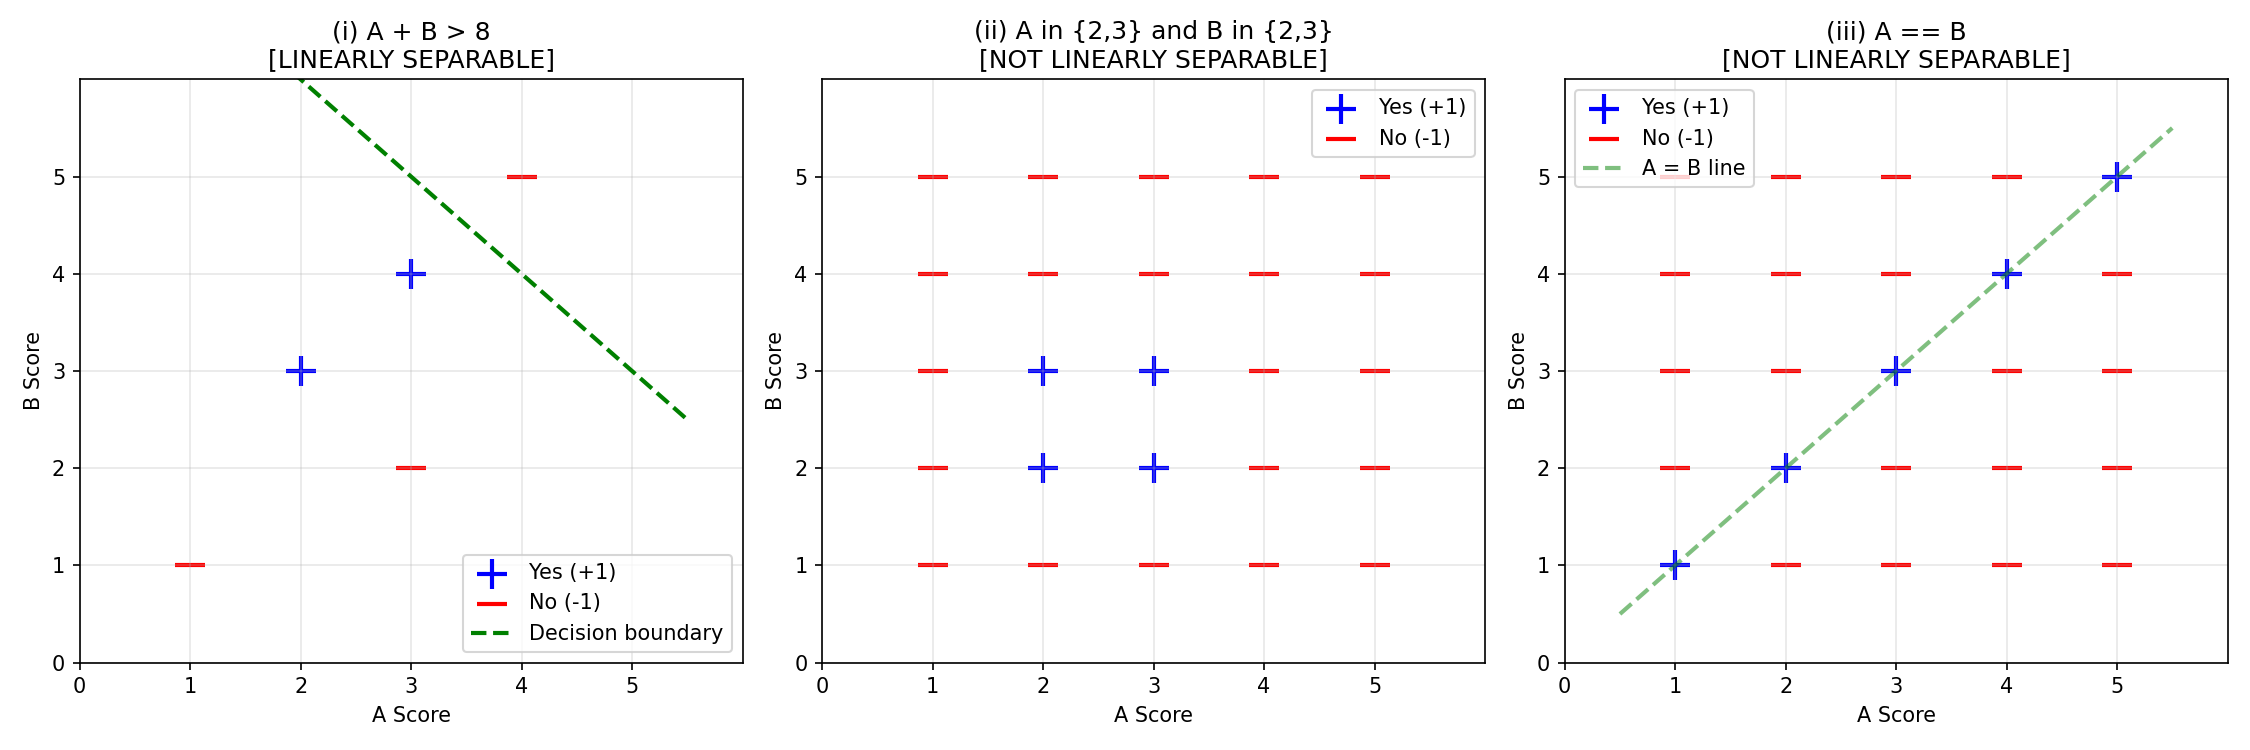
\includegraphics[width=\textwidth]{task2_scenarios.png}
    \caption{Decision boundaries for the three classification scenarios. (i) $A+B>8$ is linearly separable. (ii) $A,B \in \{2,3\}$ and (iii) $A=B$ are not linearly separable.}
    \label{fig:scenarios}
\end{figure}

\section{Task 3}

\subsection{Soft Margin SVM}

Since the dataset is not linearly separable (as shown in Task 1), a hard-margin SVM cannot find a feasible solution. We therefore apply a \textbf{soft-margin linear SVM} (implemented via \texttt{LinearSVC}) to classify the data. The soft-margin formulation introduces slack variables $\xi_i \geq 0$ that allow some training points to be on the wrong side of the margin or even the wrong side of the decision boundary. The optimization objective becomes:
\[
\min_{\mathbf{w}, b} \frac{1}{2}\|\mathbf{w}\|^2 + C \sum_{i=1}^{n} \xi_i
\]
subject to $y_i(\mathbf{w} \cdot \mathbf{x}_i + b) \geq 1 - \xi_i$ and $\xi_i \geq 0$.

\subsection{Role of the Regularization Parameter $C$}

The parameter $C > 0$ controls the trade-off between two competing goals:
\begin{itemize}
    \item \textbf{Maximizing the margin} (controlled by $\frac{1}{2}\|\mathbf{w}\|^2$): a larger margin yields better generalization and a simpler model.
    \item \textbf{Minimizing classification error} (controlled by $\sum \xi_i$): fewer misclassified training points improve training accuracy.
\end{itemize}

\begin{itemize}
    \item \textbf{Small $C$}: The penalty on misclassification is weak. The optimizer prioritizes a wide margin, even if it means accepting more training errors. The decision boundary becomes ``flatter'' and the model tends toward underfitting.
    \item \textbf{Large $C$}: The penalty on misclassification is strong. The optimizer squeezes the margin to correctly classify as many training points as possible. The boundary tilts to accommodate individual points, increasing the risk of overfitting.
\end{itemize}

\subsection{Experimental Results}

We train soft-margin linear SVMs with varying $C$ values on the movie dataset. Figure~\ref{fig:svm} shows the resulting decision boundaries.

\begin{figure}[htbp]
    \centering
    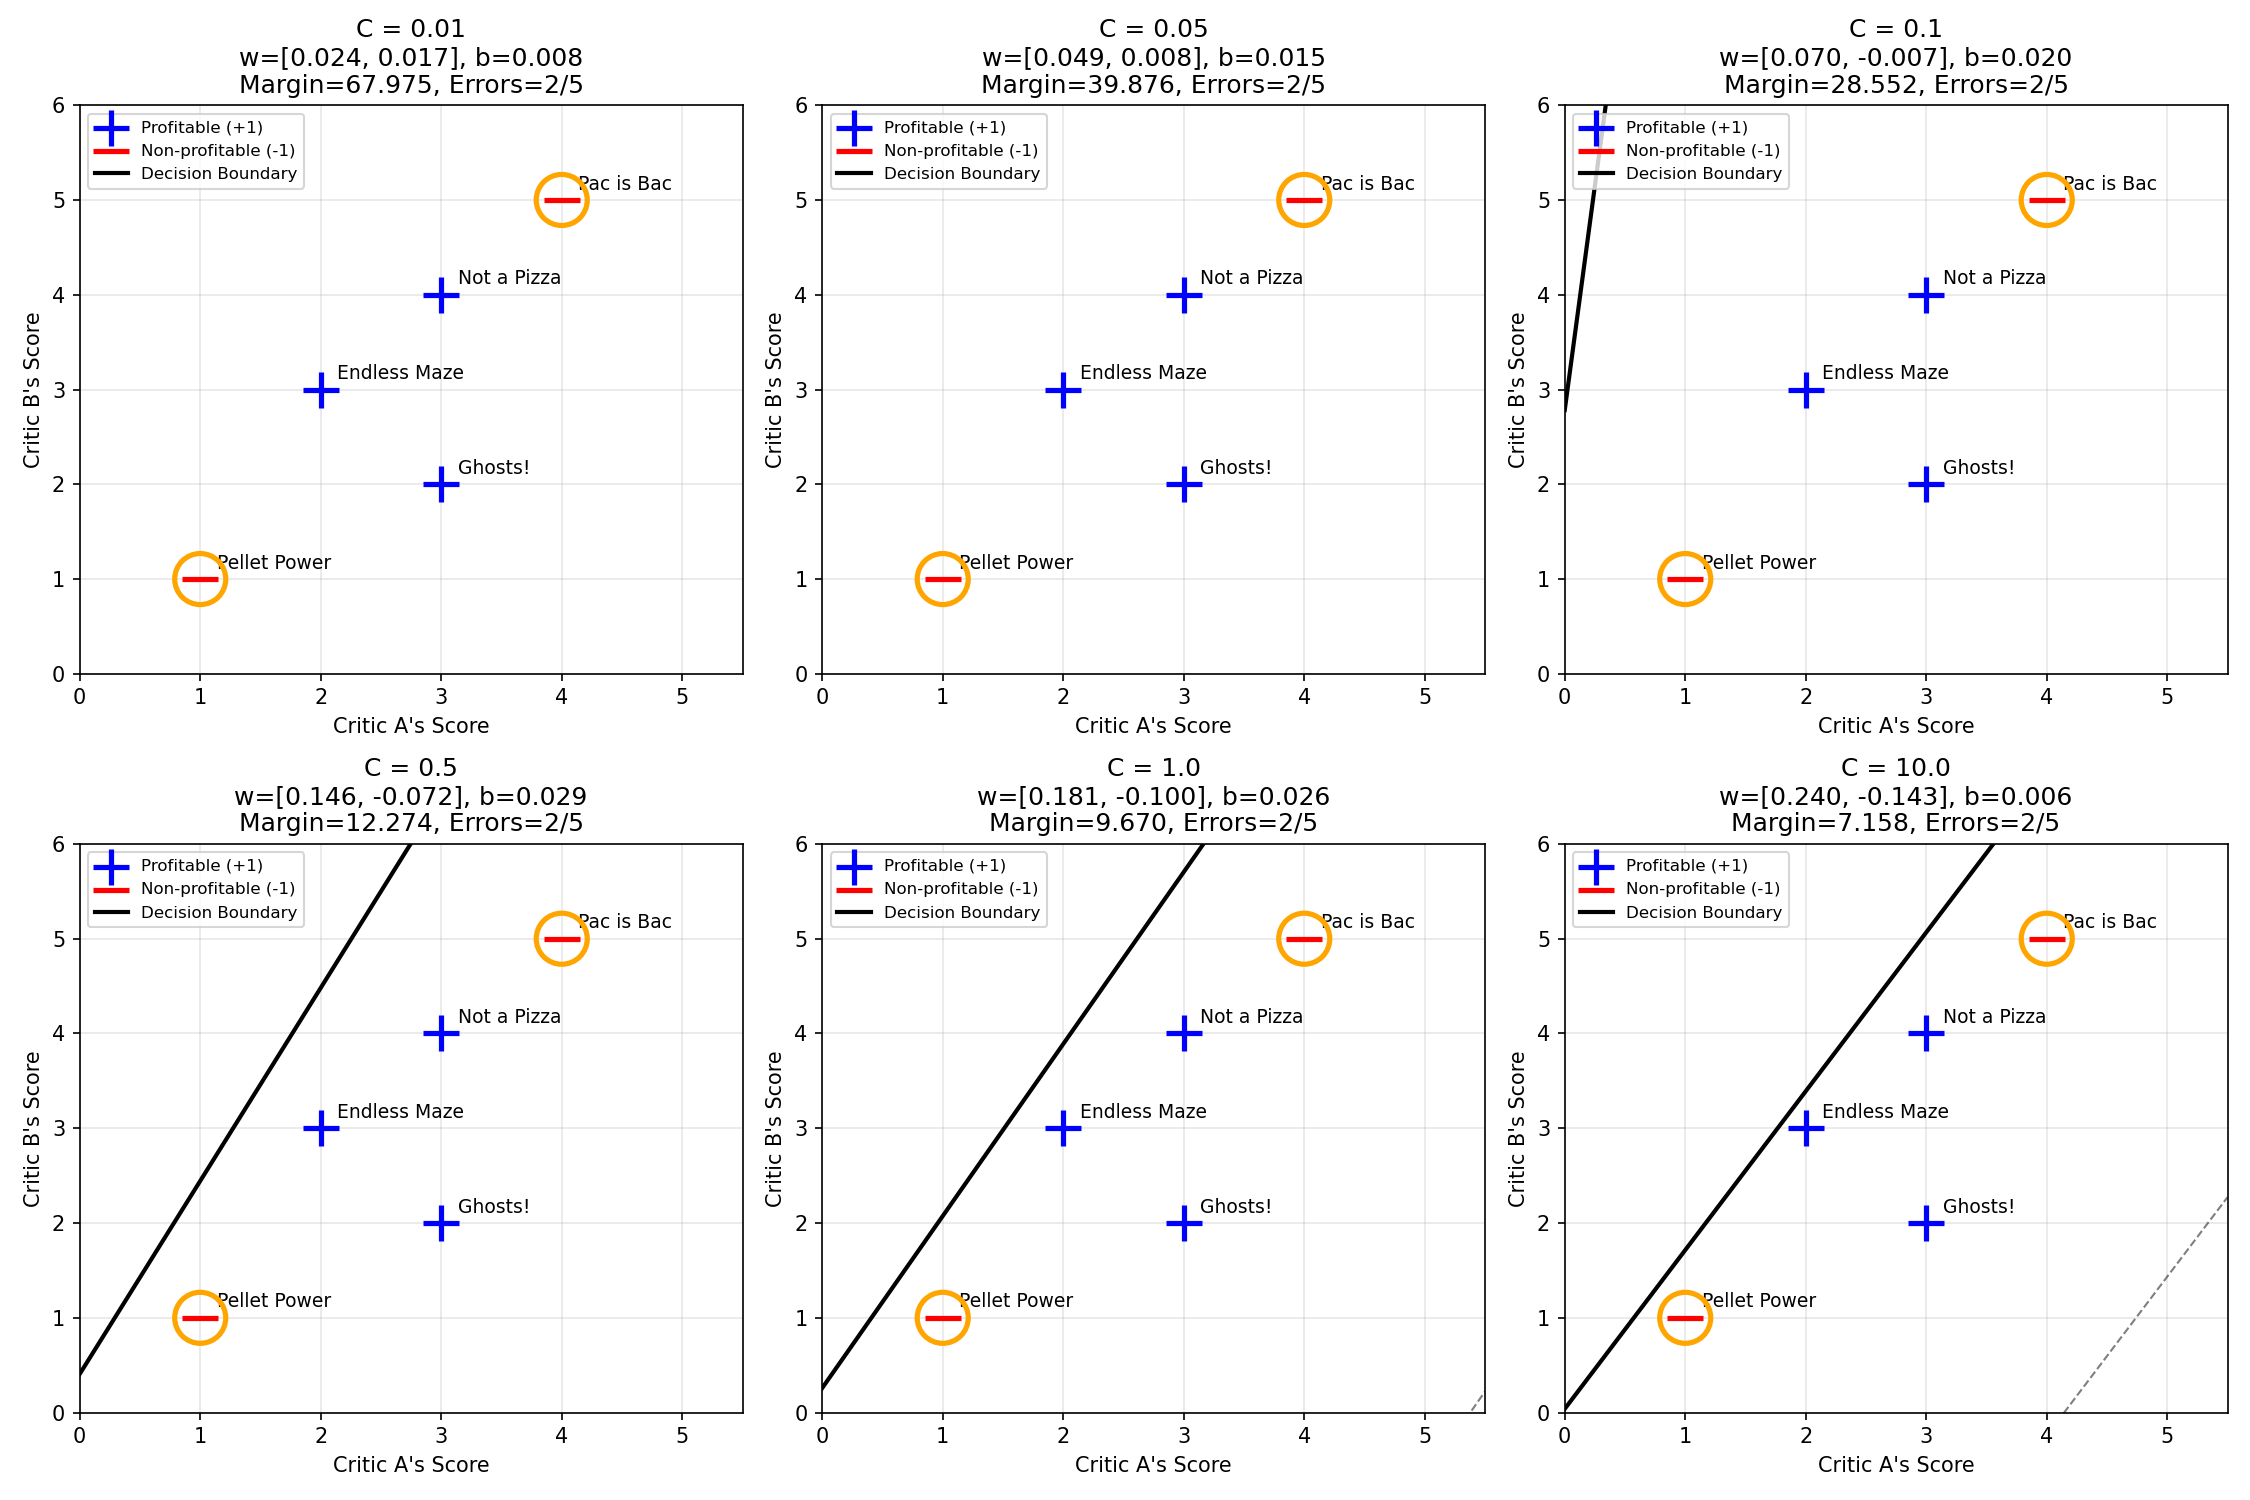
\includegraphics[width=\textwidth]{task3_svm_comparison.png}
    \caption{Soft-margin linear SVM decision boundaries for different values of $C$. Orange circles highlight misclassified points. As $C$ increases, the margin shrinks and the boundary rotates to reduce training error.}
    \label{fig:svm}
\end{figure}

\subsection{Observation and Trade-off Analysis}

Table~\ref{tab:svm} summarizes the weights, margin width, and training errors for each $C$.

\begin{table}[htbp]
\centering
\caption{Soft-margin SVM results for varying $C$.}
\label{tab:svm}
\begin{tabular}{ccccc}
\toprule
$C$ & $w_1$ & $w_2$ & Margin $2/\|\mathbf{w}\|$ & Training Errors \\
\midrule
0.01  & 0.024  & 0.017   & 67.975 & 2/5 \\
0.05  & 0.049  & 0.008   & 39.876 & 2/5 \\
0.10  & 0.070  & $-0.007$ & 28.552 & 2/5 \\
0.50  & 0.146  & $-0.072$ & 12.274 & 2/5 \\
1.00  & 0.181  & $-0.100$ & 9.670  & 2/5 \\
10.00 & 0.240  & $-0.143$ & 7.158  & 2/5 \\
\bottomrule
\end{tabular}
\end{table}

\textbf{Key observations:}
\begin{enumerate}
    \item \textbf{Persistent misclassification:} Because the data is not linearly separable, at least two points (\textit{Pellet Power} and \textit{Pac is Bac}) remain misclassified regardless of $C$.
    \item \textbf{Margin shrinks as $C$ grows:} When $C = 0.01$, the margin is very wide ($\approx 68$), reflecting the optimizer's tolerance for errors. When $C = 10$, the margin narrows to $\approx 7$ as the optimizer tries harder to classify every point correctly.
    \item \textbf{Decision boundary rotation:} With small $C$, the boundary is nearly horizontal; as $C$ increases, it tilts downward, attempting to push \textit{Pac is Bac} (the outlier at $(4,5)$) to the negative side.
\end{enumerate}

\textbf{Trade-off:} A small $C$ yields a robust, simple model with a large margin but more training errors. A large $C$ reduces training error at the cost of a smaller margin and higher model complexity. On this tiny dataset, the optimal $C$ is best chosen via cross-validation on held-out movie data rather than by training error alone.

\section{Task 4}

\subsection{Decision Tree Construction}

We build a decision tree on the same 5-point movie dataset using the standard ID3-style algorithm with \textbf{information entropy} as the splitting criterion. At each node, the tree evaluates all candidate splits and selects the one that maximizes \textbf{information gain}:
\[
\text{IG}(S, A) = H(S) - \sum_{v \in \text{Values}(A)} \frac{|S_v|}{|S|} H(S_v)
\]
where $H(S) = -\sum_{i} p_i \log_2 p_i$ is the Shannon entropy of the node.

\subsubsection{Choosing Splitting Features}

At the root node, the algorithm evaluates all possible splits on both features (A Score and B Score). The chosen split is \textbf{A Score $\leq$ 1.5}, which perfectly isolates \textit{Pellet Power} (the only non-profitable movie with A = 1) into a pure left leaf labeled \textsc{No}.

For the remaining four movies on the right branch, the next best split is \textbf{B Score $\leq$ 4.5}. This separates:
\begin{itemize}
    \item \textit{Ghosts!} (B = 2), \textit{Not a Pizza} (B = 4), and \textit{Endless Maze} (B = 3) into a pure leaf labeled \textsc{Yes}.
    \item \textit{Pac is Bac} (B = 5) into a pure leaf labeled \textsc{No}.
\end{itemize}

The resulting tree has depth 2 and 3 leaves, achieving \textbf{100\% training accuracy}. Figure~\ref{fig:tree_full} shows the complete tree structure; the entropy value in each node quantifies the remaining uncertainty before splitting.

\begin{figure}[htbp]
    \centering
    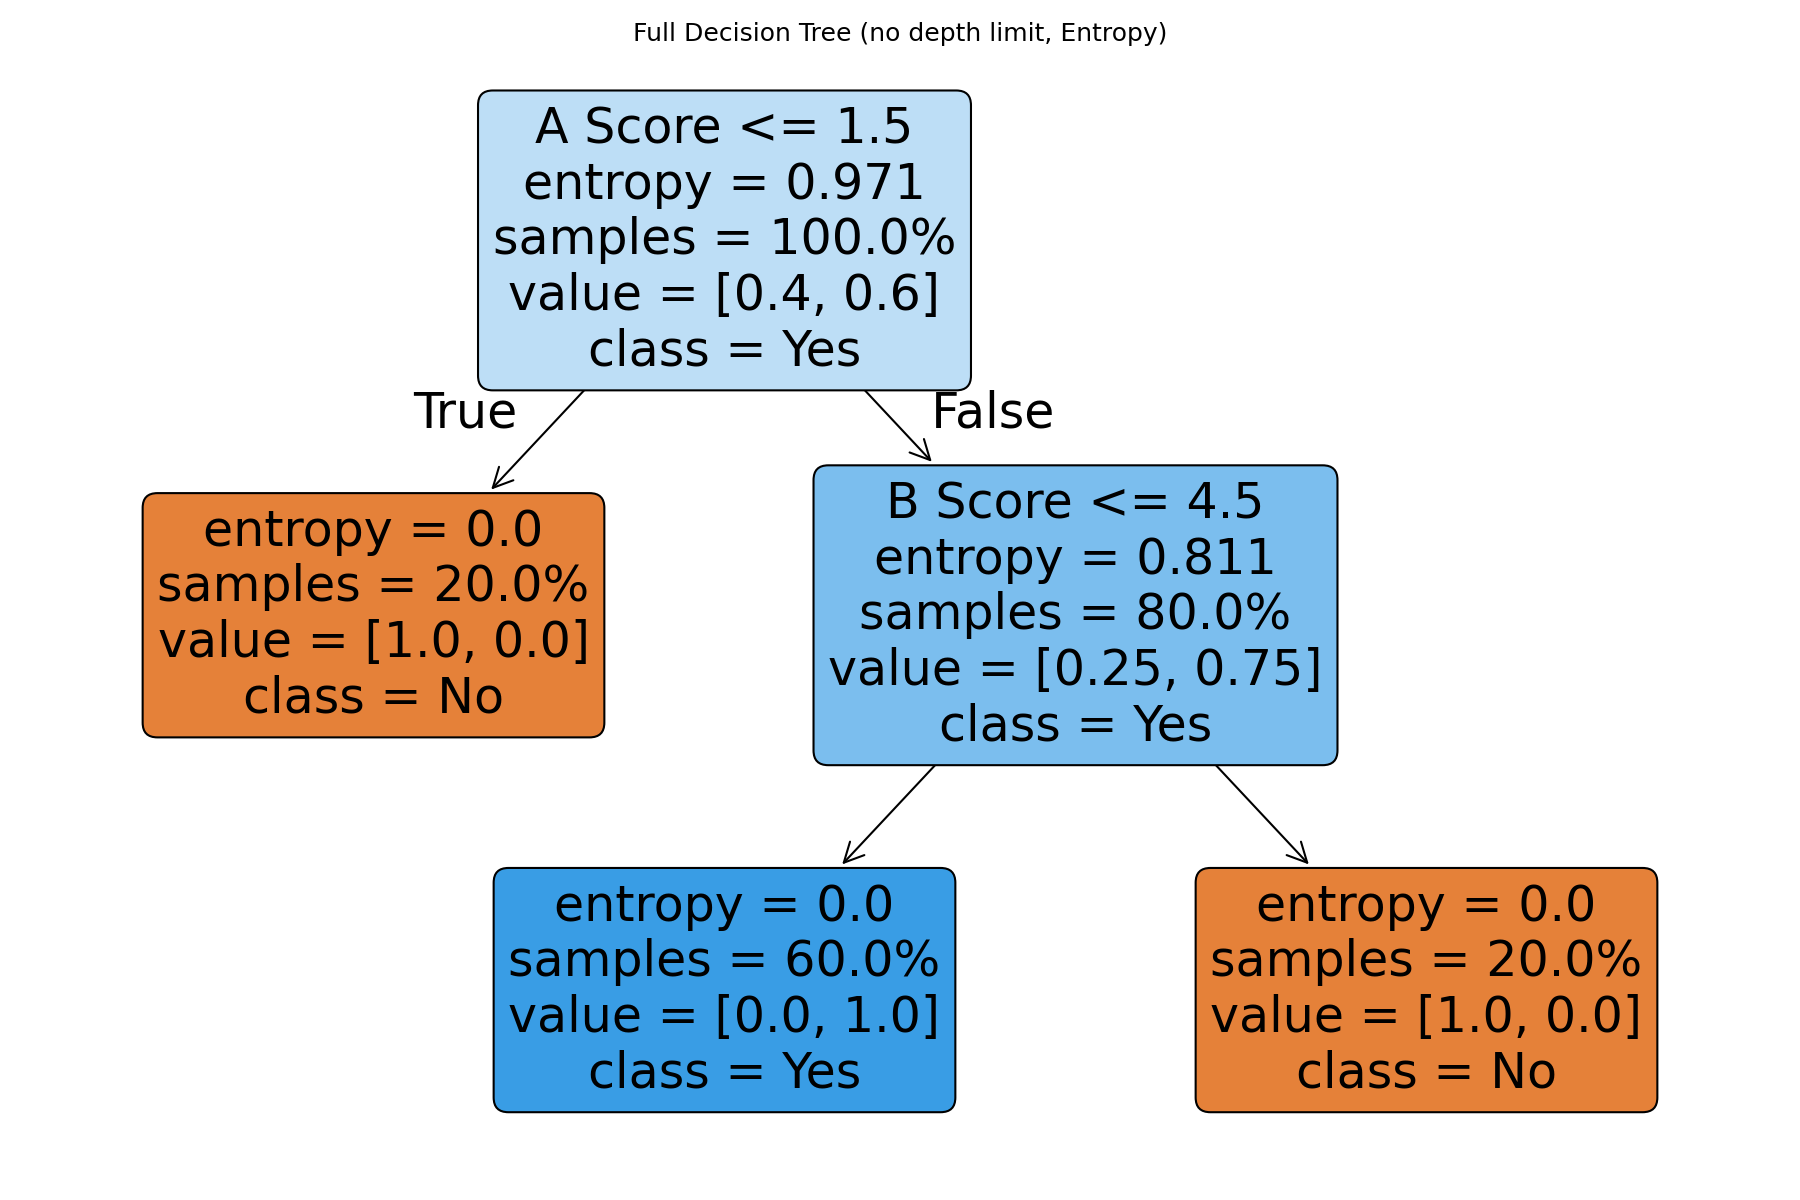
\includegraphics[width=0.85\textwidth]{task4_tree_full.png}
    \caption{Full decision tree trained on the movie dataset using entropy. The entropy value in each node measures the class uncertainty; orange nodes predict \textsc{No} and blue nodes predict \textsc{Yes}.}
    \label{fig:tree_full}
\end{figure}

\subsubsection{Feature Importance}

The computed feature importances are:
\begin{itemize}
    \item B Score: 0.6684
    \item A Score: 0.3316
\end{itemize}
B Score contributes more because the second split (B $\leq$ 4.5) resolves the remaining mixed branch and yields a larger information gain, whereas the first split only isolates a single outlier.

\subsection{Impact of Tree Depth}

Figure~\ref{fig:tree_depths} compares trees grown with different \texttt{max\_depth} limits.

\begin{figure}[htbp]
    \centering
    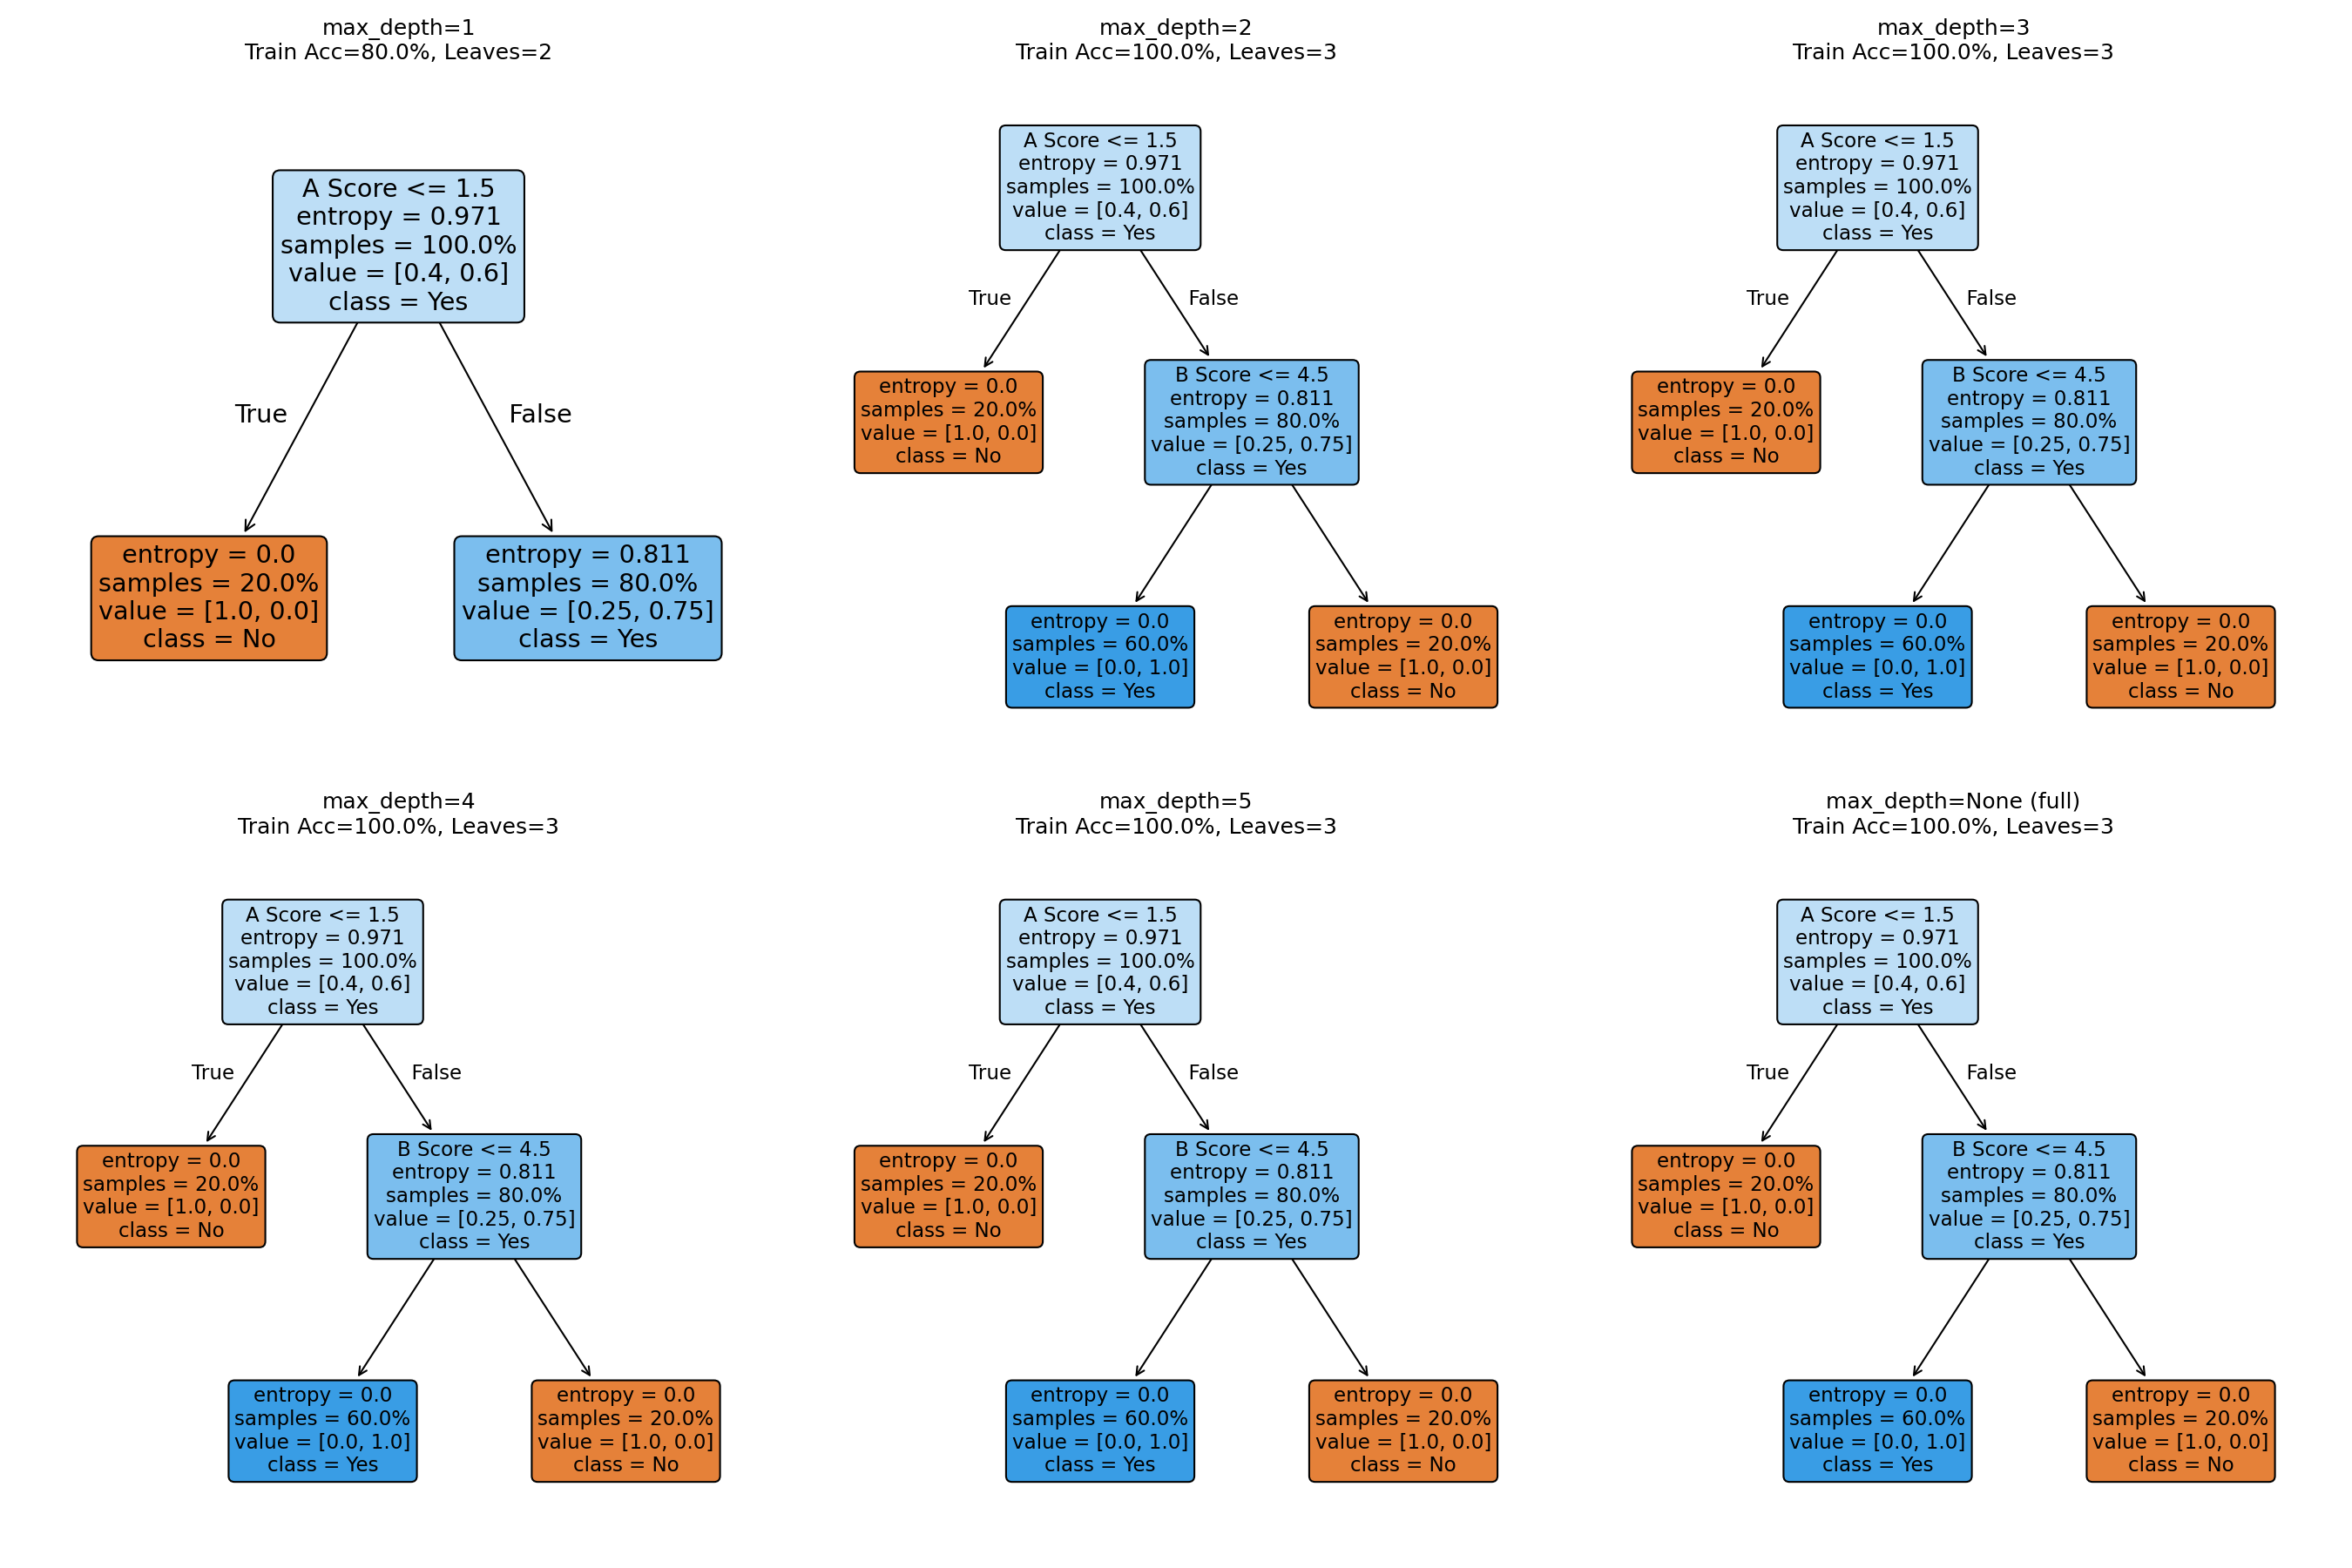
\includegraphics[width=\textwidth]{task4_tree_depths.png}
    \caption{Decision trees with varying \texttt{max\_depth} using entropy. Depth 1 yields 80\% training accuracy; depth 2 and above reach 100\%.}
    \label{fig:tree_depths}
\end{figure}

\textbf{Observations:}
\begin{itemize}
    \item \textbf{Depth 1}: Only the root split (A $\leq$ 1.5) is performed. The right leaf contains three profitable and one non-profitable movie, so it defaults to \textsc{Yes}. Training accuracy is 80\% (4/5 correct), with \textit{Pac is Bac} misclassified.
    \item \textbf{Depth 2}: The second split (B $\leq$ 4.5) is added, yielding three pure leaves with zero entropy and 100\% accuracy. This is the smallest depth that perfectly fits the training data.
    \item \textbf{Depth $\geq$ 2}: Further increases do not change the tree structure because all leaves already have zero entropy. The tree cannot overfit more even when allowed deeper splits.
\end{itemize}

\subsection{Pruning and Overfitting Prevention}

Although the full tree already achieves perfect training accuracy with only 3 leaves, pruning remains an essential technique for larger datasets. We analyze cost-complexity pruning (CCP) by varying \texttt{ccp\_alpha}. Figure~\ref{fig:tree_prune} shows the effect on tree size, total entropy, and training accuracy.

\begin{figure}[htbp]
    \centering
    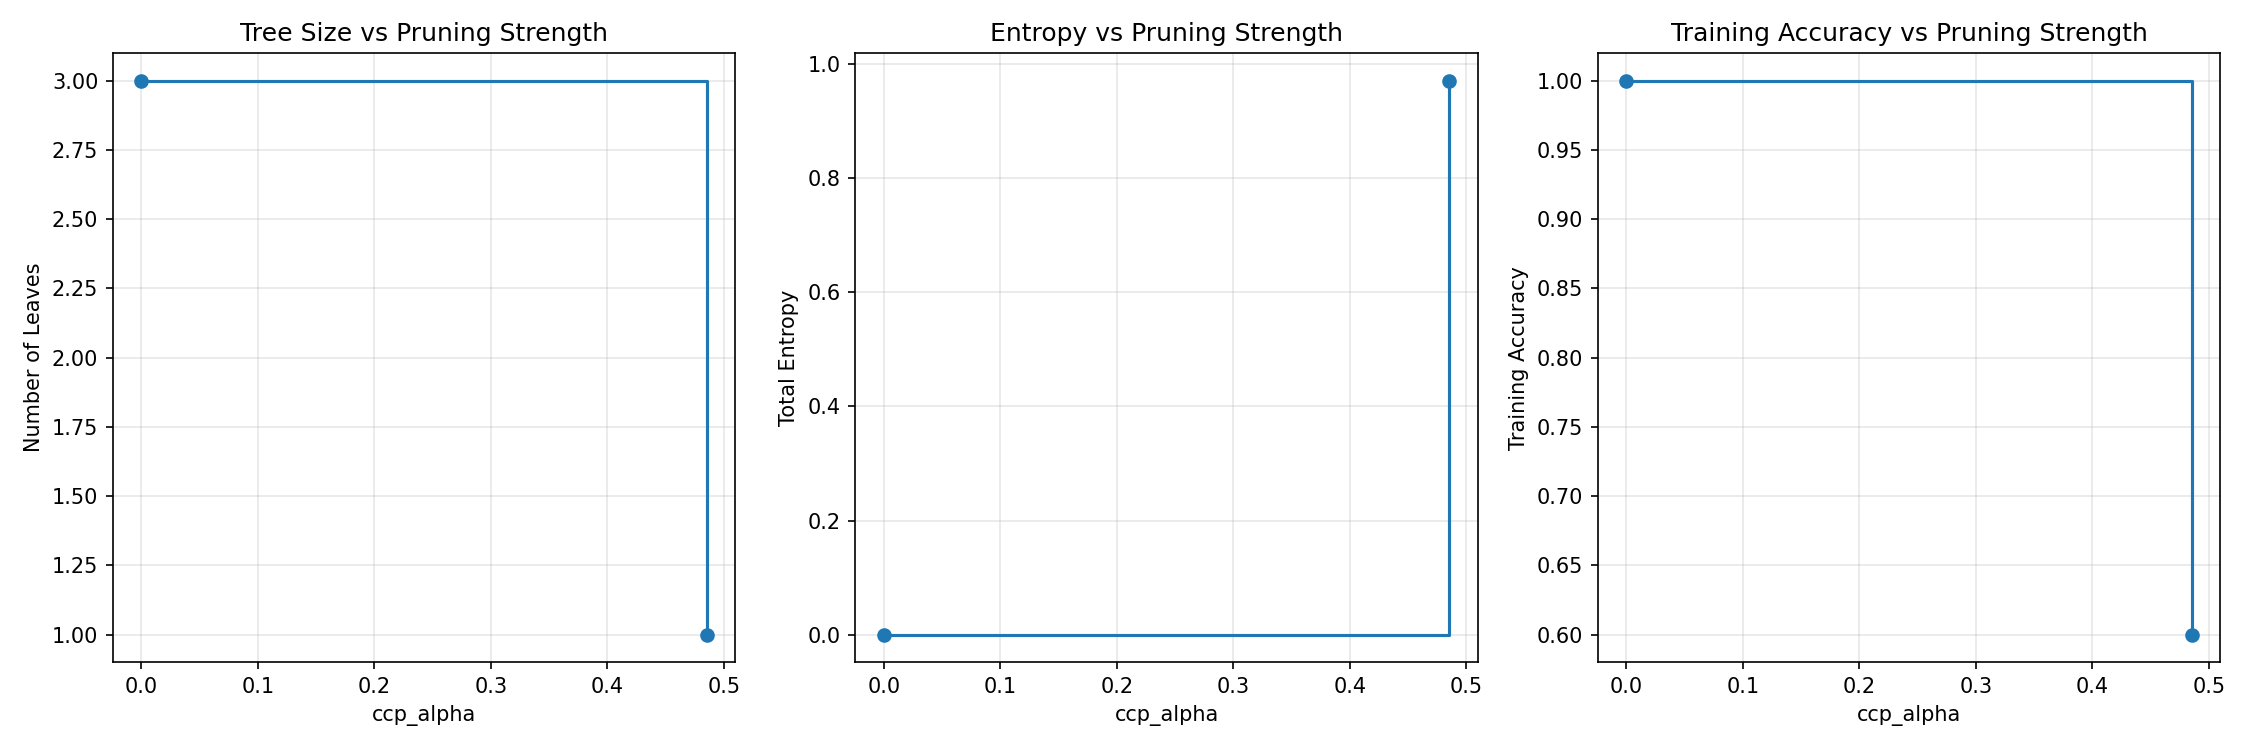
\includegraphics[width=\textwidth]{task4_tree_pruning.png}
    \caption{Effect of cost-complexity pruning on tree size, total entropy, and training accuracy.}
    \label{fig:tree_prune}
\end{figure}

\textbf{Interpretation:}
\begin{itemize}
    \item For small \texttt{ccp\_alpha} ($<$ 0.24), the tree retains 3 leaves, 0 entropy, and 100\% training accuracy.
    \item Once \texttt{ccp\_alpha} exceeds a critical value ($\approx$ 0.24), the penalty on tree complexity outweighs the benefit of entropy reduction. The tree is aggressively pruned to a single leaf, causing training accuracy to drop to 60\%.
\end{itemize}

On this tiny dataset, the unpruned tree is already parsimonious, so pruning is unnecessary. However, on larger datasets with noise, unconstrained trees can grow very deep and memorize idiosyncratic patterns. Pruning (or setting \texttt{max\_depth}, \texttt{min\_samples\_leaf}) collapses low-information branches, trading a small increase in training error for better generalization on unseen data.

\section{Task 5} 

From the previous 3 experiment, we implement the data visualization and model training using \texttt{sklearn} in Python. We compare SVM, NN(Linear Perceptron), and Decision Tree on the same dataset. The conclusion is clear: 

\begin{itemize}
    \item SVM with linear kernel fails to find a good decision boundary due to the non-linear nature of the data. The decision boundary is almost horizontal, misclassifying several points. For soft margin SVM, the decision boundary rotates as $C$ increases, but it still cannot perfectly separate the classes due to the inherent non-linearity. It is necessary to use a non-linear kernel (e.g., RBF) to capture the complex patterns in the data.
    \item NN with a single linear layer (perceptron) also fails to capture the non-linear patterns, resulting in poor classification performance. The decision boundary is a straight line that cannot separate the classes effectively. A more complex architecture (e.g., multi-layer perceptron with non-linear activation) would be needed to improve performance, but it may still struggle with such a small dataset.
    \item Decision Tree successfully captures the non-linear relationships and achieves perfect classification on the training data. The tree splits on A Score and B Score to create pure leaves, effectively separating the classes. However, it may overfit the training data, so pruning or limiting tree depth is advisable for larger datasets.
\end{itemize}

\textbf{Final Decision: } \textbf{Decision Tree} is the best choice for this dataset in terms of training accuracy and efficiency. SVM and NN (Linear Perceptron) are not suitable without modifications (e.g., non-linear kernel for SVM, deeper architecture for NN). However, for larger datasets, regularization and pruning would be necessary to prevent overfitting in Decision Trees, while SVM with an appropriate kernel and multi-layer perceptron with non-linear activation could potentially perform better.

\end{document}
